\begin{figure}[H]
\centering
    % 0b11_111
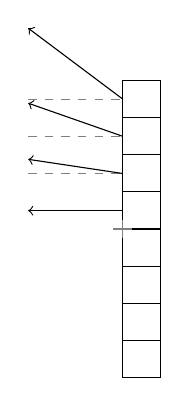
\begin{tikzpicture}[x = 1mm, y = 1mm, scale = .6]
    \begin{scope}[xshift = 20mm, local bounding box = paddle]
        \draw [black] (0, 0) rectangle ++(8, 63);

        \draw [black] (0, 7 * 63 / 8) -- ++(8, 0);
        \draw [black] (0, 6 * 63 / 8) -- ++(8, 0);
        \draw [black] (0, 5 * 63 / 8) -- ++(8, 0);
        \draw [black] (0, 4 * 63 / 8) -- ++(8, 0);
        \draw [black] (0, 3 * 63 / 8) -- ++(8, 0);
        \draw [black] (0, 2 * 63 / 8) -- ++(8, 0);
        \draw [black] (0, 1 * 63 / 8) -- ++(8, 0);
    \end{scope}

    \begin{scope}[xshift = 0, local bounding box = lines]
        % 3
        \draw [gray, -, dashed]  (0,  8 * 63 / 8 - 4) -- ++(20,  0);
        \draw [black, ->]  (20, 8 * 63 / 8 - 4) -- ++(-20, 15);
        % 2
        \draw [gray, -, dashed]  (0,  7 * 63 / 8 - 4) -- ++(20,  0);
        \draw [black, ->]  (20, 7 * 63 / 8 - 4) -- ++(-20, 7);
        % 1
        \draw [gray, -, dashed]  (0,  6 * 63 / 8 - 4) -- ++(20,  0);
        \draw [black, ->]  (20, 6 * 63 / 8 - 4) -- ++(-20, 3);
        % 0 
        \draw [gray, -, dashed]  (0,  5 * 63 / 8 - 4) -- ++(20,  0);
        \draw [black, <-] (0, 5 * 63 / 8 - 4)  -- ++(20,  0);
    \end{scope}

    \draw [gray, fill opacity = 0.5] (20, 4 * 63 / 8 + 2) -- ++(0, -4);
    \draw [gray, fill opacity = 0.5] (18, 4 * 63 / 8)     -- ++(4, 0);
    
\end{tikzpicture}
\caption{Colisões no \textit{paddle} (as setas funcionam de forma simétrica)}
\label{fig:collisions_paddle}
\end{figure}